\section{量子算法及编码实现}

对量子算法的编码实现步骤可概括为图\ref{fig_al}:
\begin{figure}[htb]
    \centering
    \caption{量子算法编码实现步骤}
    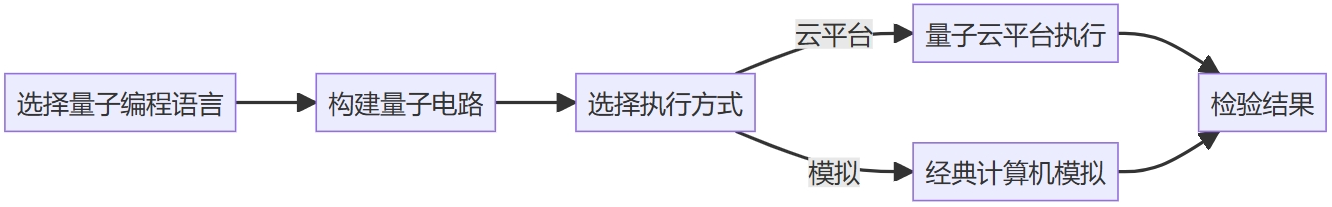
\includegraphics[width=0.9\textwidth]{figures/export.png}
    \label{fig_al}
\end{figure}

首先,需要选择一种量子编程语言,如Qiskit、Cirq、Q\#等。这些语言提供了构建量子电路、实现量子算法所需的工具和库。
之后,使用所选的量子编程语言,构建量子电路。量子电路由量子门组成,这些门定义了量子比特(qubits)之间的操作和相互作用。例如,在Qiskit中,可以使用Hadamard门和CNOT门来创建纠缠态。
构建量子电路后可以选择在真实的量子计算机上运行算法。如利用IBM Quantum、亚马逊Braket和微软Azure Quantum等平台,将构建的量子电路上传到云平台。这些平台提供量子模拟和量子硬件执行的能力,允许用户在真实的量子计算机上运行算法。
或者选择在经典计算机上模拟量子电路的运行,以验证量子算法的正确性和效率,该方法适用于小规模的量子电路。当然,由于是经典计算机上的模拟,其解决问题的实际速度不具有量子优势。
执行结束后分析算法的性能和结果。

本文通过Qiskit在计算机上模拟实现算法。
\subsection{Deutsch-Jozsa算法}
由David Deutsch和Richard Jozsa在1992年提出。该算法旨在解决所谓的Deutsch-Jozsa问题,即确定一个给定的二进制函数是常数函数还是均匀(balanced)函数。在经典计算中,确定函数是否为常数或平衡需要至少$2^{n-1}+1$次查询,其中N是函数可能输入的数量。然而,Deutsch-Jozsa算法只需一次函数查询就能解决这个问题,比任何经典算法都要快得多。
(常函数: 所有的$f(x)=0$或者1;
均匀(balanced)函数: 恰好一半$x$得$f(x) = 0$, 另一半$x$得$f(x) = 1$。)
\subsubsection{Deutsch-Jozsa算法描述}
Deutsch-Jozsa算法的量子线路如下:
\begin{define}{Deutsch-Jozsa算法量子线路}
    \begin{center}
    \begin{quantikz}[row sep=0.5cm, column sep=0.6cm]
        \lstick{$\ket{0}^{\otimes n}$} & \qw & \gate{H^{\otimes n}} & \qw & 
        \gate[2][2.0cm]{U_f}\gateinput[1]{$x$}\gateoutput[1]{$x$} & \qw & \gate{H^{\otimes n}} & \meter{} \\
        \lstick{$\ket{0}$} & \gate{X} & \gate{H} & \qw & \gateinput{$y$}\gateoutput{$y\oplus f(x)$} & \qw & \qw & \qw
    \end{quantikz}
    \end{center} 
\end{define}

$U_f$称为量子黑箱(Oracle),定义为:
$$
    U_f:\ket{x,y}\rightarrow\ket{x,y\oplus f(x)}
$$

若$|y\rangle = \frac{|0\rangle - |1\rangle}{\sqrt{2}}$,则有
$$
\begin{aligned}
    U_f : &|x\rangle \left( \frac{|0\rangle - |1\rangle}{\sqrt{2}} \right) \mapsto \left( \frac{U_f |x\rangle |0\rangle - U_f |x\rangle |1\rangle}{\sqrt{2}} \right)\\
    &= |x\rangle \left| 0 \oplus f(x) \right\rangle - |x\rangle \left| 1 \oplus f(x) \right\rangle\\
    &= |x\rangle \left( \frac{|0 \oplus f(x)\rangle - |1 \oplus f(x)\rangle}{\sqrt{2}} \right)
\end{aligned}
$$

当 $f(x) =$ 0 或 1 时,有
\[
\begin{cases} 
    f(x) = 0: & \frac{|0 \oplus f(x)\rangle - |1 \oplus f(x)\rangle}{\sqrt{2}} = \frac{|0\rangle - |1\rangle}{\sqrt{2}} \\ 
    f(x) = 1: & \frac{|0 \oplus f(x)\rangle - |1 \oplus f(x)\rangle}{\sqrt{2}} = \frac{|1\rangle - |0\rangle}{\sqrt{2}} = -\frac{|0\rangle - |1\rangle}{\sqrt{2}} 
\end{cases} 
\]

\[ \frac{|0 \oplus f(x)\rangle - |1 \oplus f(x)\rangle}{\sqrt{2}} = (-1)^{f(x)} \left( \frac{|0\rangle - |1\rangle}{\sqrt{2}} \right) \]

可见,$U_f$作用于 $|x\rangle \left( \frac{|0\rangle - |1\rangle}{\sqrt{2}} \right)$相当于从整体上添加了一个相位因子 $(-1)^{f(x)}$。

\[ U_f : |x\rangle \left( \frac{|0\rangle - |1\rangle}{\sqrt{2}} \right) \mapsto (-1)^{f(x)} |x\rangle \left( \frac{|0\rangle - |1\rangle}{\sqrt{2}} \right) \]

Deutsch-Jozsa算法工作过程如下:

1. 输入态: $|0\rangle^{\otimes n} \otimes |1\rangle$

2. $H^{\otimes n+1}$变换:

\[
|\psi_1\rangle = \left( \frac{|0\rangle + |1\rangle}{\sqrt{2}} \right)^{\otimes n} \otimes \frac{|0\rangle - |1\rangle}{\sqrt{2}} = \sum_{x \in \{0,1\}^n} \frac{|x\rangle\rangle}{\sqrt{2^n}} \otimes \frac{|0\rangle - |1\rangle}{\sqrt{2}}
\]

3. $\hat{U}$变换:

\[
|\psi_2\rangle = \hat{U}|\psi_1\rangle = \sum_{x \in \{0,1\}^n} \frac{(-1)^{f(x)}|x\rangle\rangle}{\sqrt{2^n}} \otimes \frac{|0\rangle - |1\rangle}{\sqrt{2}}
\]

4. $H^{\otimes n}$变换:

由 $H|y\rangle = \sum_{z=0,1} \frac{(-1)^{yz}}{\sqrt{2}} |z\rangle (y = 0 \text{和} 1)$ 得
\[
|\psi_3\rangle = \hat{U}|\psi_1\rangle = \sum_{x,z \in \{0,1\}^n} \frac{(-1)^{f(x) + x \cdot z}|z\rangle}{2^n} \otimes \frac{|0\rangle - |1\rangle}{\sqrt{2}}
\]

其中 $x \cdot z = \sum_{i=1}^{n} x_i z_i \mod 2$

5. 测量:

若 $f(x)$ 为常函数,则 $|z\rangle = |0\rangle^{\otimes n}$ 的系数为 $\sum_{x \in \{0,1\}^n} \frac{(-1)^{f(x)}}{2^n} = \pm 1$,此时 $|\psi_3\rangle = |0\rangle^{\otimes n} \otimes \frac{|0\rangle - |1\rangle}{\sqrt{2}}$,所以测量结果为所有量子位均为0。

若 $f(x)$ 为均匀函数,则 $|z\rangle = |0\rangle^{\otimes n}$ 的系数为零,所以测量结果不可能所有的量子位均为0。

\subsubsection{Deutsch-Jozsa算法Qiskit实现}
\bold{1.实现黑盒函数}

定义函数 \texttt{dj\_oracle(case, n)} 实现 Oracle,并将其构建为一个名为 Oracle 的自定义门,返回参数为新构建的自定义门的标识符。参数 $n$ 为输入量子比特的数目。参数 \texttt{case} 为字符串类型:当 \texttt{case} 为 \texttt{"constant"} 时,实现了常值函数;当 \texttt{case} 为 \texttt{"balanced"} 时,实现了平衡函数。
\begin{py}
\begin{lstlisting}
## oracle函数
def dj_oracle(case, n):
    oracle_qc = QuantumCircuit(n+1)
    # 平衡函数
    if case == "balanced":
        # [1,2**n)间的随机整数 b
        b = np.random.randint(1, 2**n)
        # 得到 b 对应的二进制字符串
        b_str = format(b, '0'+str(n)+'b')
        # 若b_str[qubit]为'1',则在q[qubit]上添加一个X门
        for qubit in range(len(b_str)):
            if b_str[qubit] == '1':
                oracle_qc.x(qubit)
        # 每个量子比特上添加 CNOT 门,q[n]为目标量子比特
        for qubit in range(n):
            oracle_qc.cx(qubit, n)
        # 若b_str[qubit]为'1',则在q[qubit]上添加一个X门
        for qubit in range(len(b_str)):
            if b_str[qubit] == '1':
                oracle_qc.x(qubit)

    # 常值函数
    if case == "constant":
        # 取随机整数0或1, 若为1,则在q[n]上添加一个X门
        output = np.random.randint(2)
        if output == 1:
            oracle_qc.x(n)

    oracle_gate = oracle_qc.to_gate()
    # 将量子线路 oracle_qc 封装为自定义门
    oracle_gate.name = "Oracle"
    return oracle_gate
\end{lstlisting}
\end{py}

例如,当$n=3$,$b=3$时利用以下代码可以得到平衡函数对应的量子线路:
\begin{py}
\begin{lstlisting}
from qiskit import QuantumCircuit 
import numpy as np
n = 3
oracle_qc = QuantumCircuit(n+1)
b = 3
b_str = format(b, '0'+str(n)+'b')
for qubit in range(len(b_str)):
    if b_str[qubit] == '1':
        oracle_qc.x(qubit)
for qubit in range(n):
    oracle_qc.cx(qubit, n)
for qubit in range(len(b_str)):
     if b_str[qubit] == '1':
        oracle_qc.x(qubit)
         
print(b_str)
oracle_qc.draw(output='mpl',filename='qc2.png')#获得png图片
\end{lstlisting}
\end{py}
\fig{平衡函数量子线路}{0.6}{code/qc2.png}
$q_0$,$q_1$ 和 $q_2$ 为输入量子比特,$q_3$ 为辅助量子比特。易知,输入为000、011、101、110时$q_3$进行了两次“非”,即$q_3$保持不变,对应$f(x)$为0。输入为111、001、100、010时$q_3$进行了一次或三次“非”,对应$f(x)$为1。故$f(x)$为平衡函数。

\bold{2.实现Deutsch-Jozsa算法的量子线路}
\begin{py}
\begin{lstlisting}
def dj_algorithm(oracle, n):
    dj_circuit = QuantumCircuit(n+1, n)
    # 设置输出量子比特
    dj_circuit.x(n)
    dj_circuit.h(n)
    # 设置输入寄存器
    for qubit in range(n):
        dj_circuit.h(qubit)
    # 添加 Oracle 门
    dj_circuit.append(oracle, range(n+1))
    # 输入寄存器各量子比特上添加 H 门
    for qubit in range(n):
        dj_circuit.h(qubit)
    # 测量输入寄存器
    for i in range(n):
        dj_circuit.measure(i, i)
    return dj_circuit



# 库函数输入
import numpy as np
from qiskit_aer import Aer
from qiskit import QuantumCircuit, transpile
from qiskit.visualization import plot_histogram

#实现4量子比特 Deutsch-Jozsa 算法量子线路
n = 4
oracle_gate = dj_oracle('constant', n)
# 平衡函数时,'constant'改为 'balanced'

dj_circuit = dj_algorithm(oracle_gate, n)
#dj_circuit.draw(output='mpl',filename='qc3.png')#获得png图片
\end{lstlisting}
\end{py}
\fig{4量子比特 Deutsch-Jozsa 算法量子线路图}{0.6}{code/qc3.png}

\bold{3.模拟运行Deutsch-Jozsa算法}
\begin{py}
\begin{lstlisting}
# 选择模拟器
simu = Aer.get_backend('aer_simulator')

# 编译运行电路
transpiled_dj_circuit = transpile(dj_circuit, simu)
results = simu.run(transpiled_dj_circuit).result()

# 获取测量结果
answer = results.get_counts(dj_circuit)
plot_histogram(answer)
\end{lstlisting}
\end{py}
测试结果测得 $|0000\rangle$ 的概率为 100\%对应 $f(x)$ 是常值函数。
测试结果测得 $|1111\rangle$ 的概率为 100\%对应 $f(x)$ 是平衡函数。(由于代码实现平衡函数时对其进行了限制,其他的态没有出现。)
\fig{常函数Deutsch-Jozsa 算法结果}{0.8}{code/const.png}
\fig{平衡函数Deutsch-Jozsa 算法结果}{0.8}{code/balanced.png}
\subsection{Grover搜索算法}
Grover搜索算法是由Lov Grover在1996年提出的一种量子算法,它主要用于解决无序数据库搜索问题,即在一个无序的数据库中寻找特定的元素。Grover算法被认为是继Shor算法之后的第二大量子算法,也是第一个被完整实验实现的量子算法。求解无序数据库搜索问题(假设只有一个目标搜索数据),经典算法所需的时间复杂度为\(\mathcal{O}(N)\),而Grover搜索算法所需的时间复杂度仅为\(\mathcal{O}(\sqrt{N})\),相比经典算法具有平方加速,展示了量子计算的强大性能。
\subsubsection{Grover搜索算法描述}
Grover算法的基本原理是利用量子叠加和量子干涉来放大目标态的概率振幅,同时抑制非目标态的概率振幅,这个过程被称为振幅放大。通过这种方式,Grover算法能够在多项式时间内找到一个无序数据库中的所有匹配项。
算法完成的任务: 一未知的黑盒$f :\{0,1\}^n\rightarrow\{0,1\}$, 找出使得$f(x) = 1$的$x$。

Grover算法的量子线路如下:
\begin{define}{Grover算法量子线路}
    \begin{center}
        \begin{quantikz}
            \lstick{$\ket{0}^{\otimes n}$} & \gate{H^{\otimes n}} & \gate[wires=2]{\hat{G}} & \gate[wires=2]{\hat{G}} & \qw \cdots & \gate[wires=2]{\hat{G}} & \meter{} \\
            \lstick{$\ket{1}$} & \gate{H} & \qw & \qw & \qw \cdots & \qw & \qw
        \end{quantikz}
    \end{center}

\begin{center}
    \begin{quantikz}
        \qw  & \gate[2][1cm]{\hat{G}} & \qw \\
        \qw & \qw & \qw
    \end{quantikz}$\Rightarrow$
    \begin{quantikz}
        \lstick{\ket{\psi}} & \qwbundle[n=2]{n} & \gate[2][1.7cm]{U_f}\gateinput[1]{$x$}\gateoutput[1]{$x$}  & \gate{2\ket{\psi}\bra{\psi} - I} & \qw \\
        \lstick{$\frac{\ket{0} - \ket{1}}{\sqrt{2}}$}& \qw & \gateinput{$y$}\gateoutput{$y\oplus f(x)$}  & \qw & \qw  \\
    \end{quantikz}    
\end{center}
\end{define}

Grover算法工作过程如下:

首先对初态为 $|0\rangle^{\otimes n}$,用 Hadamard 变换 $H^{\otimes n}$ 得到等权叠加态 $|\psi\rangle$(包含所有搜索问题的解与非搜索问题的解),即
\[
|\psi\rangle = \frac{1}{\sqrt{N}} \sum_{x=0}^{N-1} |x\rangle
\]

其中,$N = 2^n$。

此后,Grover算法连续多次执行G迭代操作。

Grover 的一次迭代分为以下四步:
\begin{enumerate}
    \item 执行 Oracle 操作($U_f$ 算符),将搜索问题的解对应的索引态增加相位因子 $-1$。
    \item Hadamard 变换 $H^{\otimes n}$。
    \item 相位变换:保持基态 $|0\rangle$ 的系数不变,其他基态的系数增加一个负号,对应的算符记为 $U_0 = 2|0\rangle\langle 0| - I$。
    \item Hadamard 变换 $H^{\otimes n}$。
\end{enumerate}

将2、3、4结合后的效果为
\[
U_{\psi} = H^{\otimes n} U_0 H^{\otimes n} = H^{\otimes n} (2|0\rangle\langle 0| - I) H^{\otimes n}
\]
\[
= 2H^{\otimes n} |0\rangle\langle 0| H^{\otimes n} - I = 2|\psi\rangle\langle\psi| - I
\]

于是,Grover 一次迭代的操作算符 $G$ 等价于
\[
G = U_{\psi} U_f = (2|\psi\rangle\langle\psi| - I) U_f
\]

通过上面的迭代,测量塌缩到索引的态的概率增大,多次迭代后完成搜索。
\subsubsection{Grover算法Qiskit实现}
通过Qiskit实现$\ket{000},\ket{001},\ket{100},\ket{010},\ket{011},\ket{110},\ket{101},\ket{111}$找$\ket{111}$的Grover算法。

Qiskit实现:

\bold{1.实现黑盒函数}

\begin{py}
\begin{lstlisting}
# 初始化
import numpy as np
# 导入 Qiskit 库
from qiskit import QuantumCircuit, transpile, quantum_info
from qiskit_aer import QasmSimulator
from qiskit import ClassicalRegister, QuantumRegister
from qiskit.visualization import plot_histogram

# 设置量子比特数量
n = 3

# 定义 Oracle 函数,用于标记特定的量子态 |111>
def Oracle():  
    oc = QuantumCircuit(n) 
    # 使用H门和CCX门(受控非门)来实现 CZ 门的效果
    oc.h(2)  # 对第2个量子比特应用Hadamard门
    oc.ccx(0, 1, 2)  # 应用受控非门
    oc.h(2)  # 再次对第2个量子比特应用Hadamard门
    return oc

\end{lstlisting}
\end{py}

\bold{2.实现振幅放大}

\begin{py}
\begin{lstlisting}
# 定义扩散算子函数,用于实现幅度放大
def A(nb): 
    ac = QuantumCircuit(nb)
    ac.h(range(nb))  # 对所有量子比特应用Hadamard门
    ac.x(range(nb))  # 对所有量子比特应用X门(非门)
    # 执行多控制Z门
    ac.h(nb-1)  # 对最后一个量子比特应用Hadamard门
    ac.mcx(list(range(nb-1)), nb-1)  # 多控制Z门
    ac.h(nb-1)  # 再次对最后一个量子比特应用Hadamard门
    ac.x(range(nb))  # 对所有量子比特应用X门
    ac.h(range(nb))  # 对所有量子比特再次应用Hadamard门
    return ac
\end{lstlisting}
\end{py}

\bold{3.实现Grover算法}
\begin{py}
\begin{lstlisting}
    # 创建量子电路
    qc = QuantumCircuit(n)
    qc.h(range(n))  # 对所有量子比特应用Hadamard门
    
    # 构建 Oracle 和幅度放大电路
    OA = QuantumCircuit(n)
    # 将Oracle函数内的内容组合到OA电路中
    OA.compose(Oracle(), inplace=True)  
    # 将扩散算子组合到OA电路中
    OA.compose(A(n), inplace=True)  
    # 将OA电路组合到qc电路中
    qc.compose(OA, inplace=True)     
    # 绘制电路图
    qc.draw(output='mpl',filename='grover_circuit.png')
\end{lstlisting}
\end{py}
\fig{Grover算法量子电路}{0.8}{code/grover_circuit.png}

\bold{4.模拟运行}
\begin{py}
\begin{lstlisting}
qc.save_statevector()  # 保存量子电路的状态向量


simulator = QasmSimulator()
compiled_circuit = transpile(qc, simulator)
job = simulator.run(compiled_circuit, shots=1000)
result = job.result()  # 获取运行结果
out_state = result.get_statevector()  # 获取状态向量
counts = result.get_counts()  # 获取测量结果的计数
# 反转字典 counts 中的字符串并存储到新字典answer中
answer = {}
for str in counts:
    answer[str[::-1]] = counts[str]  
# 绘图
plot_histogram(answer).savefig('groverout.png') 
\end{lstlisting}
\end{py}
\fig{Grover算法输出结果}{0.5}{code/groverout.png}
从输出结果不难看出,$\ket{111}$的振幅(出现的概率)被明显放大,代码实现了Grover算法的功能。